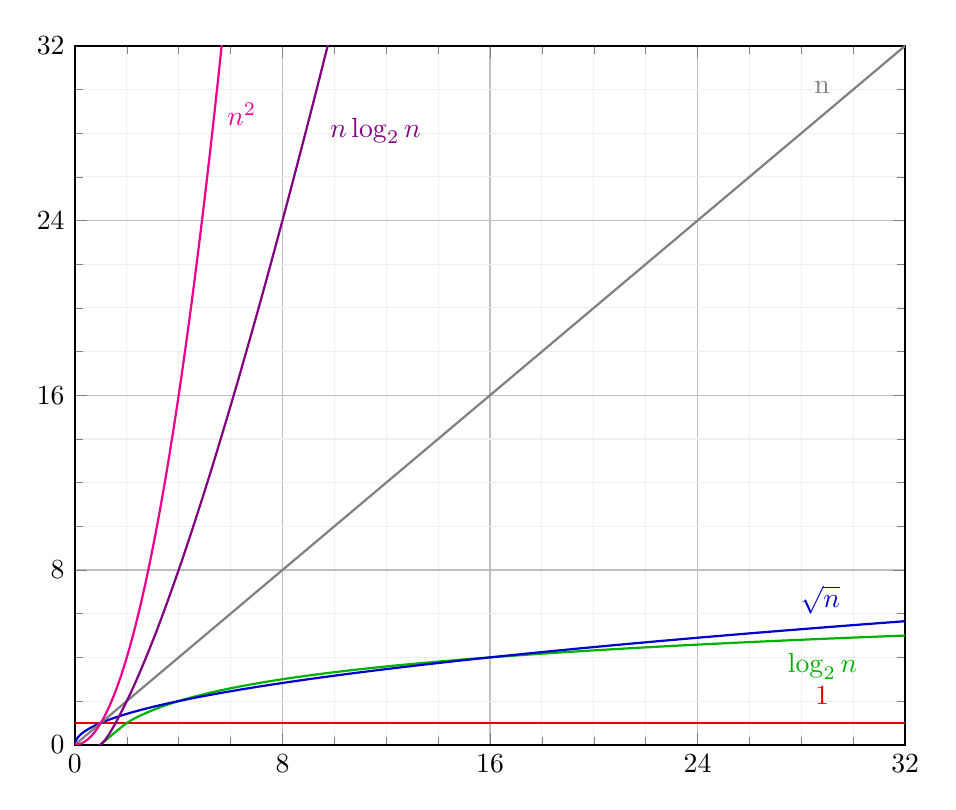
\begin{tikzpicture}
    \begin{axis}[
        width = \hsize, thick, smooth,
        domain = 0:32, xmin = 0, xmax = 32, ymin = 0, ymax = 32,
        xtick distance = 8, ytick distance = 8,
        minor tick num = 3,
        grid = both,
        major grid style = {lightgray},
        minor grid style = {lightgray!25},
        legend cell align = left,
    ]
        \addplot[red!90!black] {1}
            [yshift=1em] node [pos=0.9] {1};
        \addplot[green!70!black, samples = 32] {log2(x)}
            [yshift=-1em] node [pos=0.9] {$\log_{2}n$};
        \addplot[blue!80!black, samples = 512] {sqrt(x)}
            [yshift=1em] node [pos=0.9] {$\sqrt{n}$};
        \addplot[gray] {x}
            [yshift=1em] node [pos=0.9] {n};
        \addplot[violet, samples = 32] {x * log2(x)}
            [xshift=2em,yshift=-2em] node [pos=0.2] {$n \log_{2}n$};
        \addplot[magenta, samples = 128] {x * x}
            [xshift=1em] node [pos=0.029] {$n^2$};
    \end{axis}
\end{tikzpicture}
